\begin{tikzpicture}[
    every node/.style={node distance=0,
                       font=\small},
    label/.style={yshift=1mm},
    row label/.style={anchor=base west, xshift=-1cm, font=\normalsize}
]
    % \node (gui) {
    %     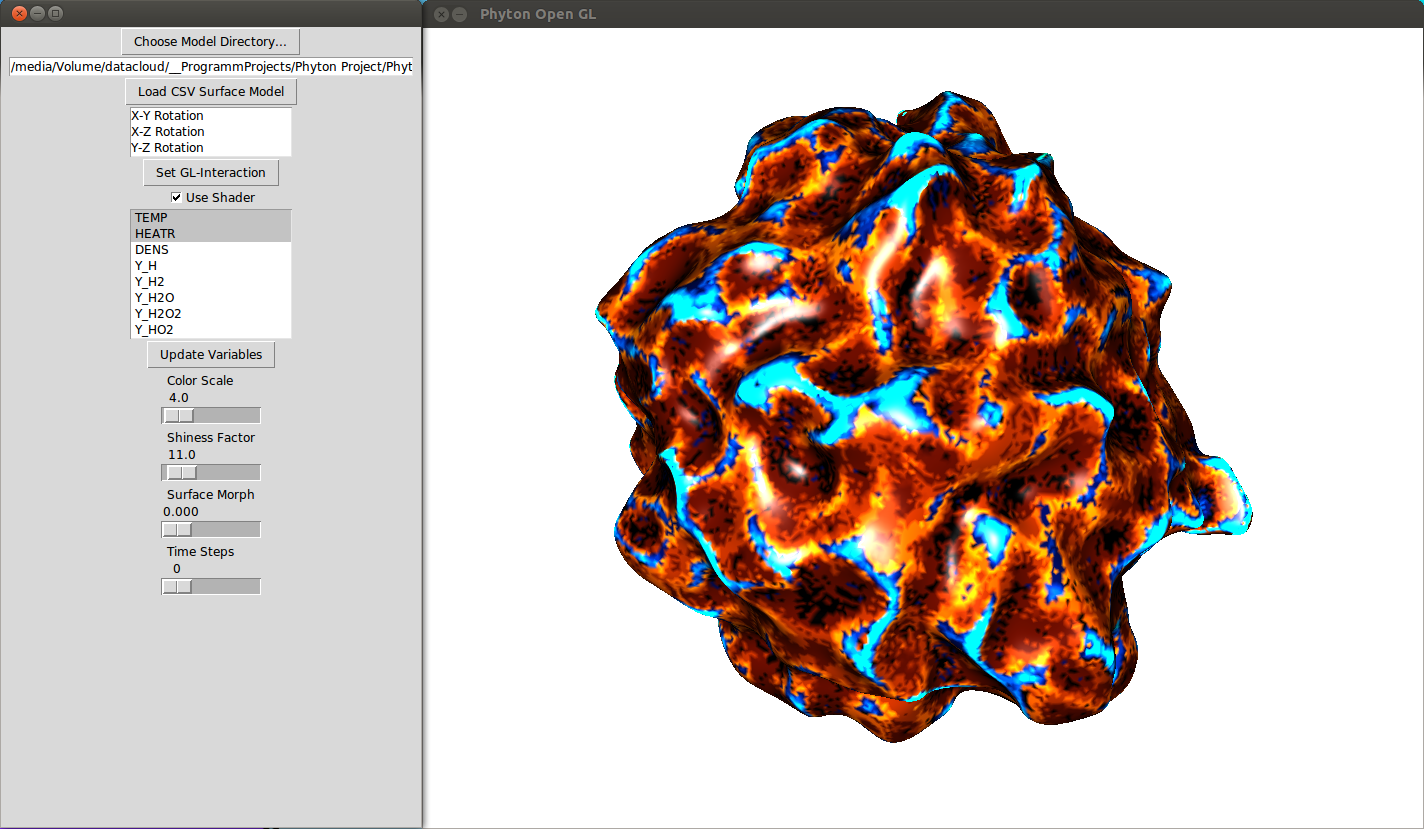
\includegraphics[width=0.5\figurewidth]{figures/sr_gui.png}
    % };

    \matrix[matrix of nodes,] (cs) {
        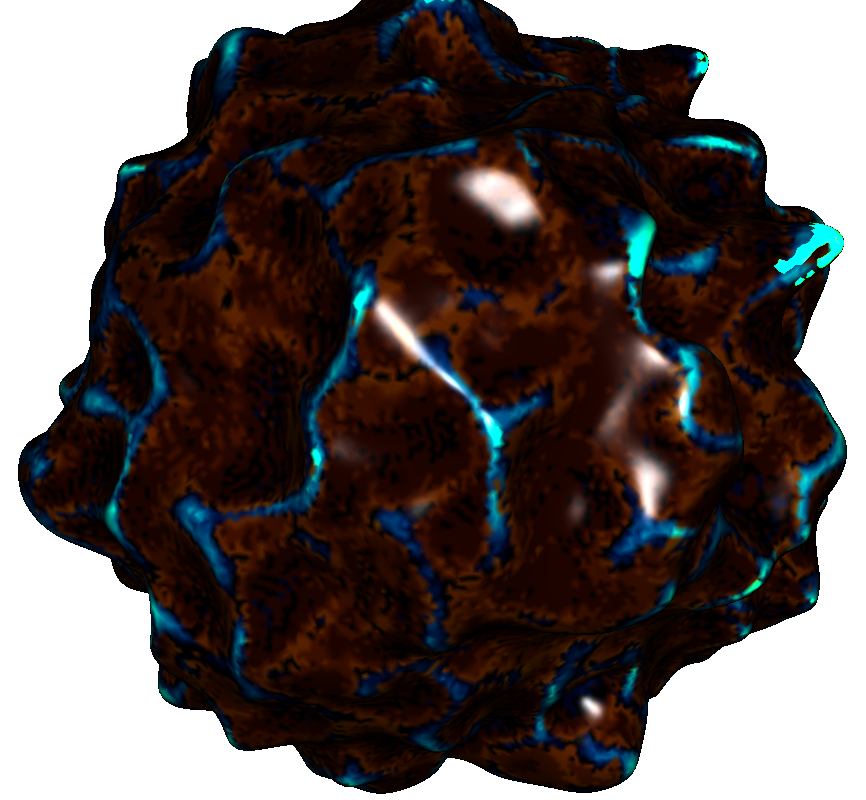
\includegraphics[width=0.22\figurewidth]{figures/sr_colorscale_1.png} &
        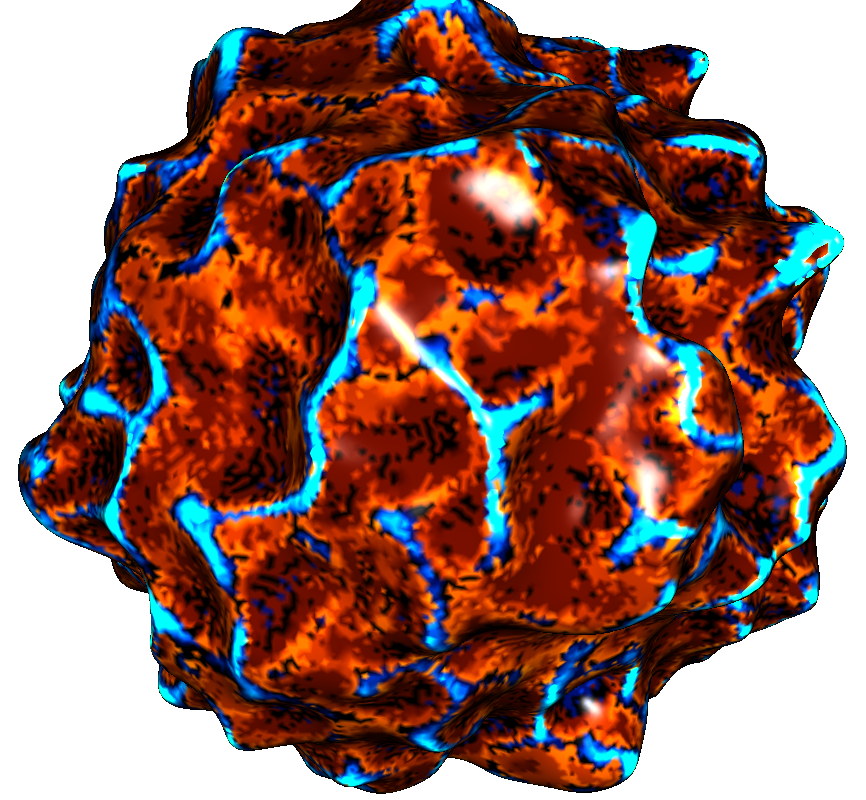
\includegraphics[width=0.22\figurewidth]{figures/sr_colorscale_2.png} &
        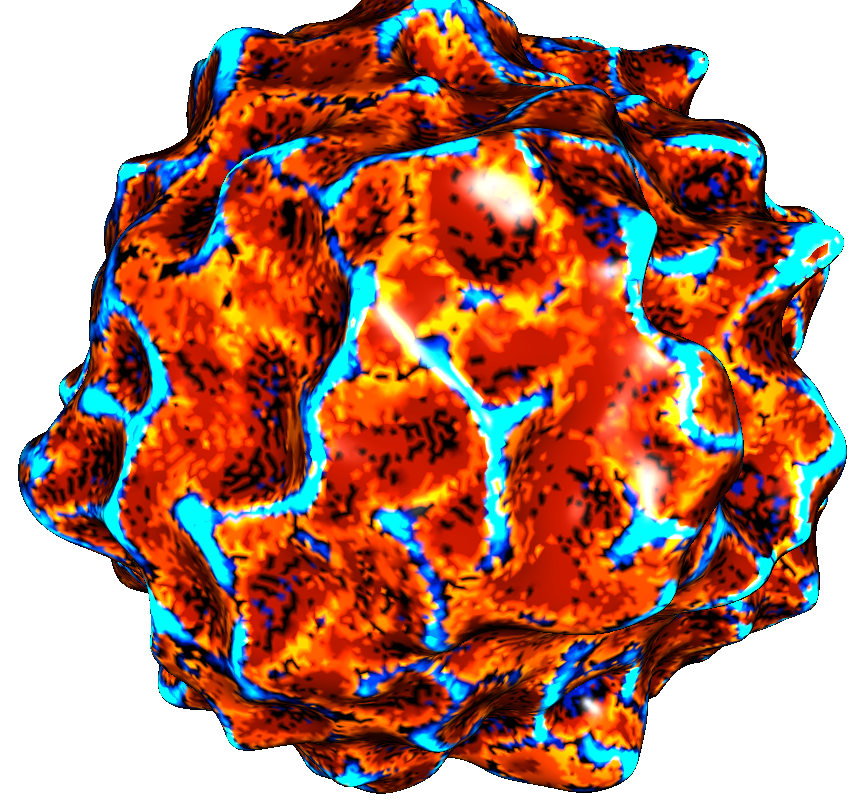
\includegraphics[width=0.22\figurewidth]{figures/sr_colorscale_3.png} \\
    };
    \node[label, below=of cs-1-1] {$u_1=1$};
    \node[label, below=of cs-1-2] {$u_1=2.5$};
    \node[label, below=of cs-1-3] {$u_1=4$};

    % \draw[thick] ([xshift=-1cm]cs.south west) -- (cs.south east);
    \node[row label, at=(cs.north west)] {color scale};
    \node[left=of cs] {
        \rotatebox{90}{$t^\textnormal{TEMP}_\textnormal{infl}$
                       vs. $t^\textnormal{HEATR}_\textnormal{max}$}
    };

    \matrix[matrix of nodes, below=1cm of cs] (morph) {
        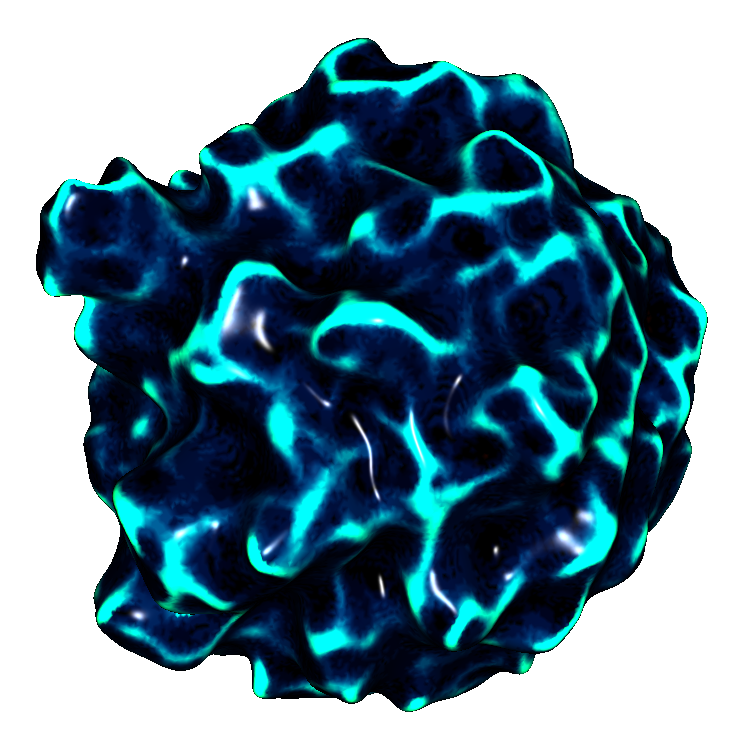
\includegraphics[width=0.22\figurewidth]{figures/sr_morphing_1.png} &
        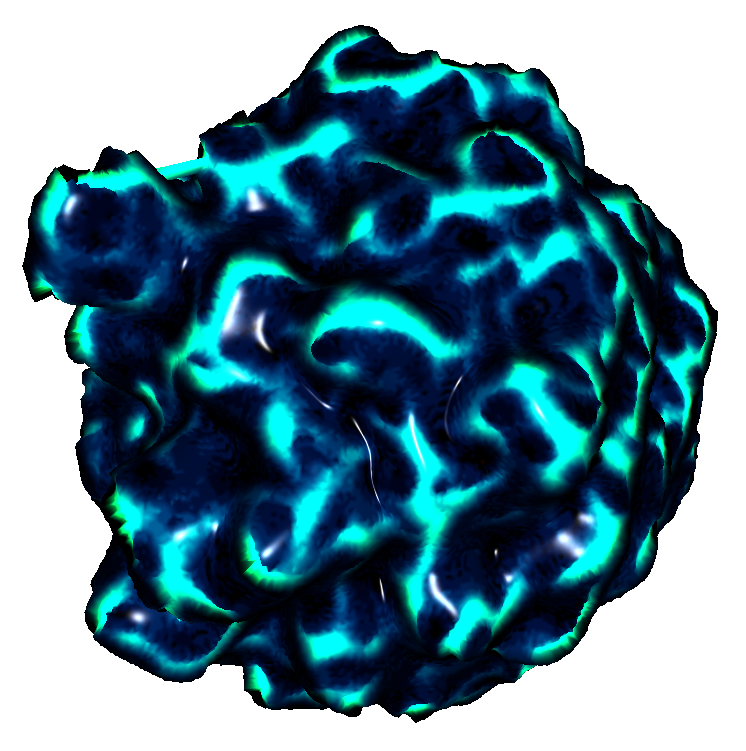
\includegraphics[width=0.22\figurewidth]{figures/sr_morphing_2.png} &
        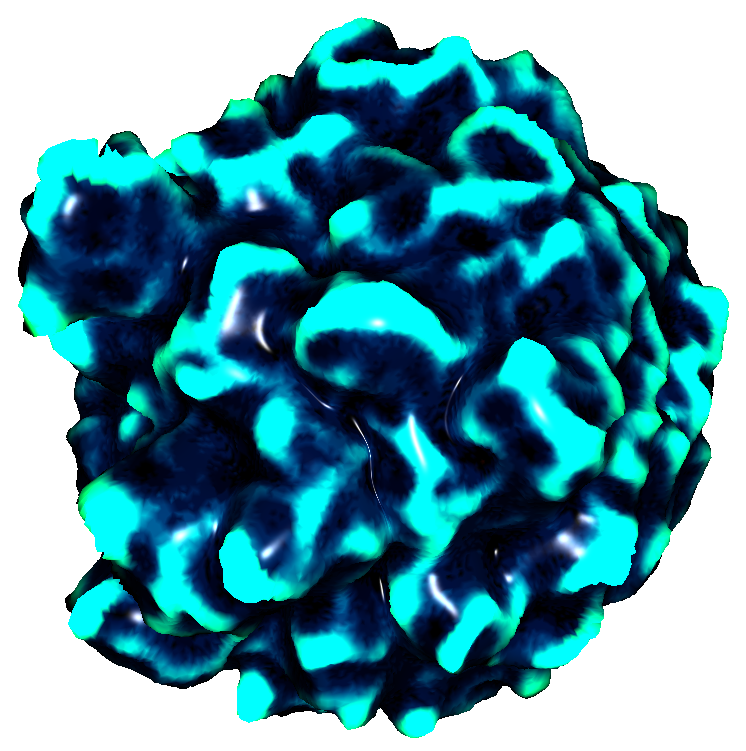
\includegraphics[width=0.22\figurewidth]{figures/sr_morphing_3.png} \\
    };
    \node[label, below=of morph-1-1] {$u_2=0$};
    \node[label, below=of morph-1-2] {$u_2=1$};
    \node[label, below=of morph-1-3] {$u_2=2$};

    % \draw[thick] ([xshift=-1cm]morph.south west) -- (morph.south east);
    \node[row label, at=(morph.north west)] {morphing};
    \node[left=of morph] {
        \rotatebox{90}{$t^\textnormal{HEATR}_\textnormal{max}$
                       vs. $t^{\ce{H2O2}}_\textnormal{max}$}
    };

    \matrix[matrix of nodes, below=1cm of morph] (time) {
        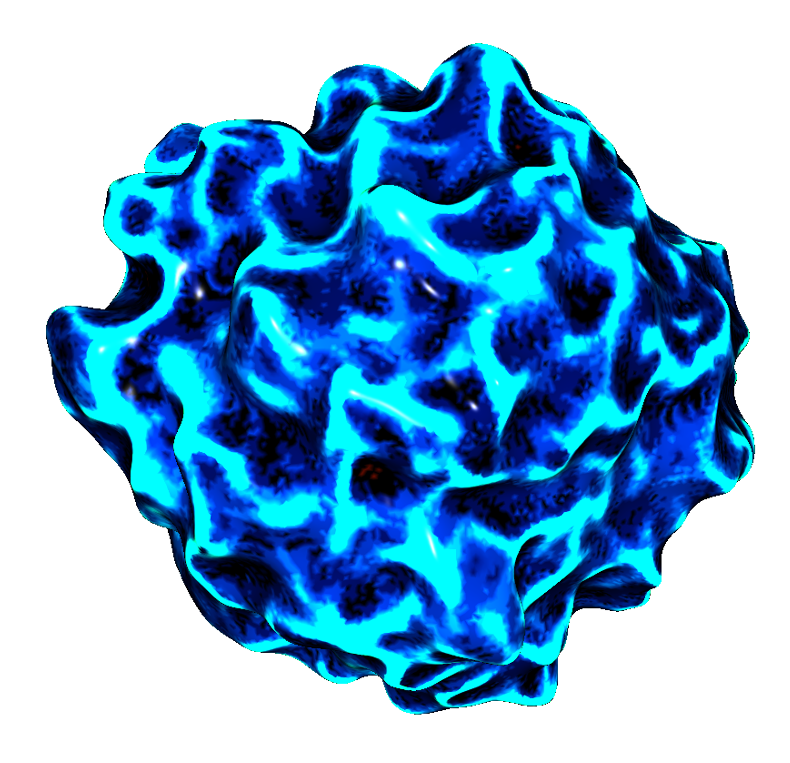
\includegraphics[width=0.22\figurewidth]{figures/sr_time_1_1.png} &
        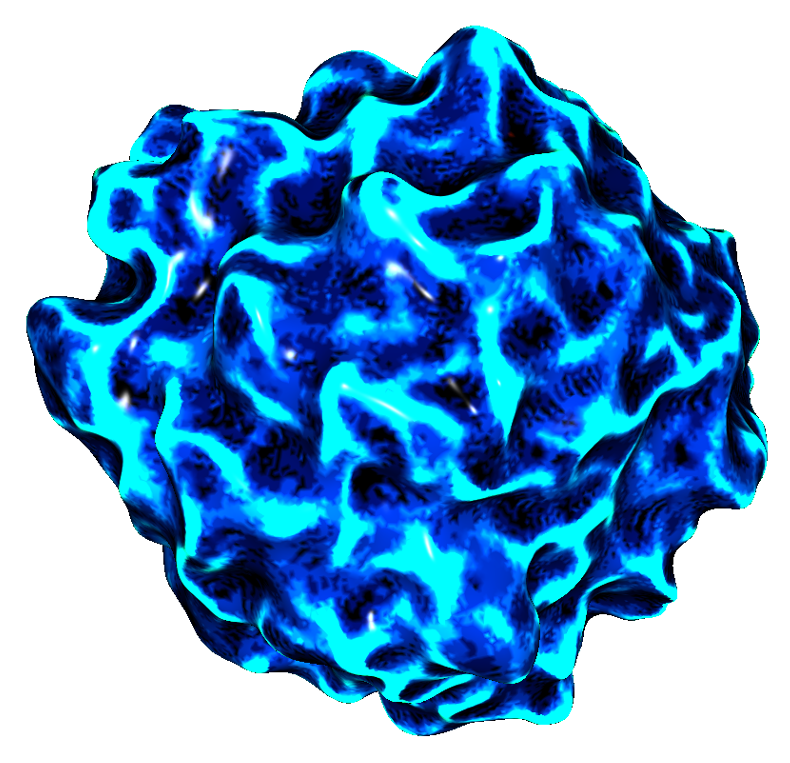
\includegraphics[width=0.22\figurewidth]{figures/sr_time_1_2.png} &
        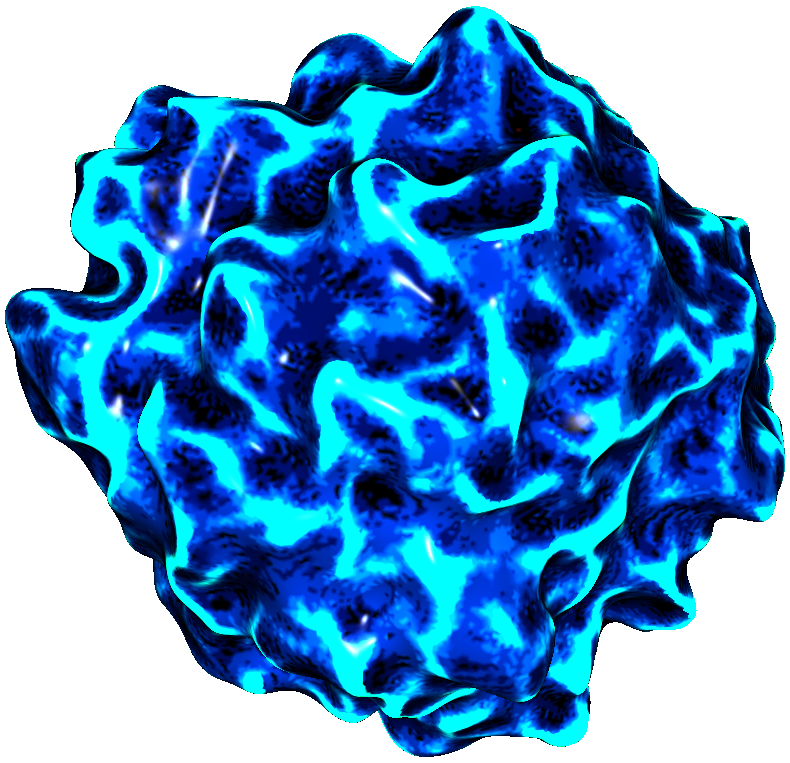
\includegraphics[width=0.22\figurewidth]{figures/sr_time_1_3.png} \\
        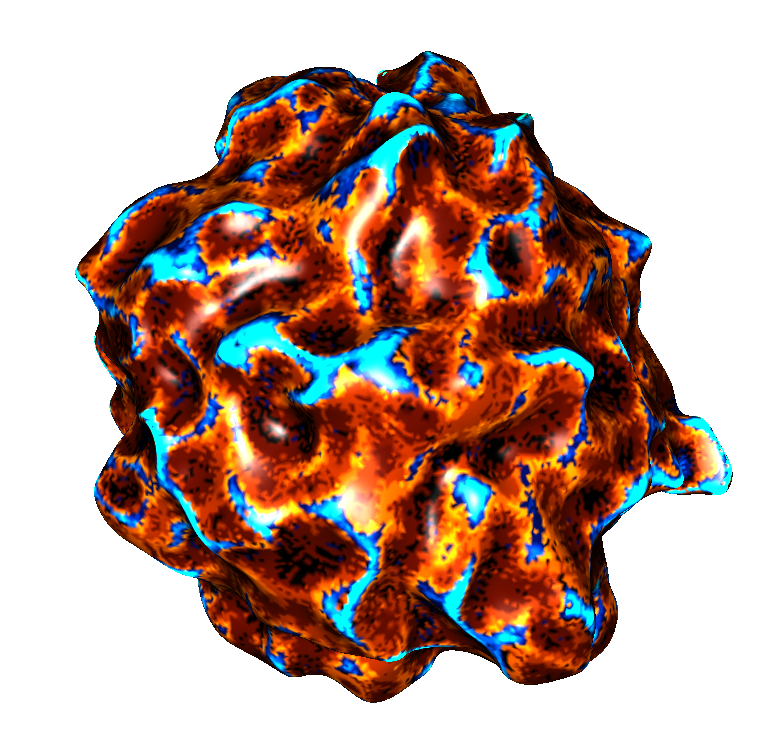
\includegraphics[width=0.22\figurewidth]{figures/sr_time_2_1.png} &
        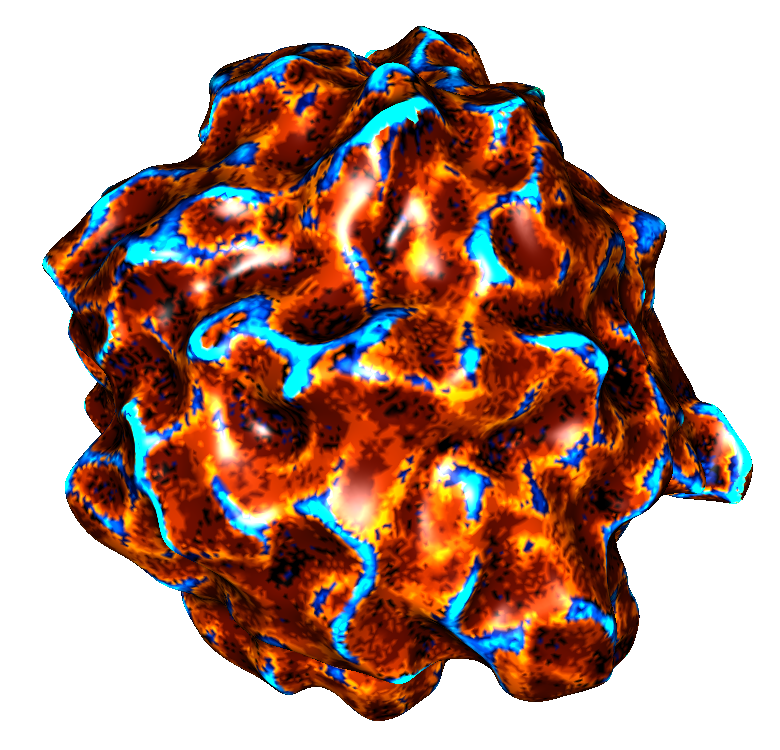
\includegraphics[width=0.22\figurewidth]{figures/sr_time_2_2.png} &
        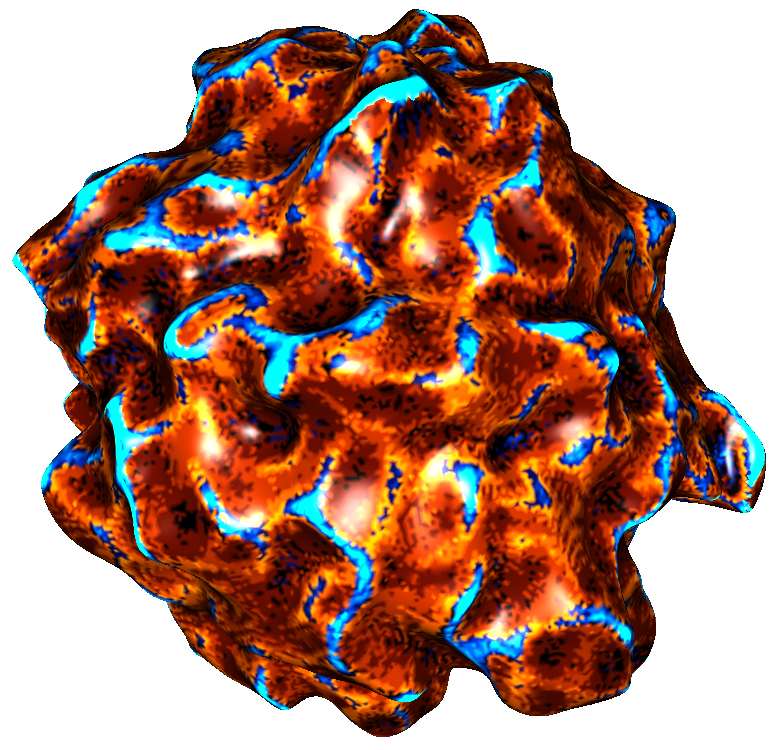
\includegraphics[width=0.22\figurewidth]{figures/sr_time_2_3.png} \\
        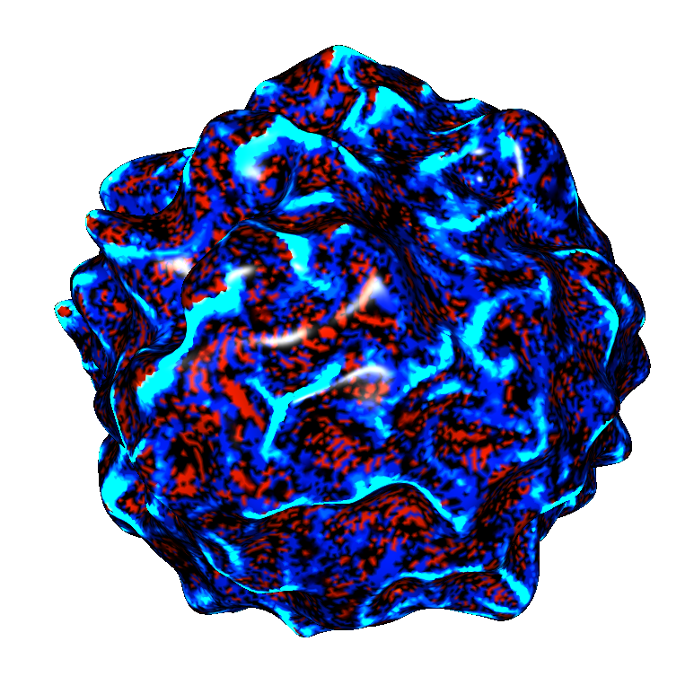
\includegraphics[width=0.22\figurewidth]{figures/sr_time_3_1.png} &
        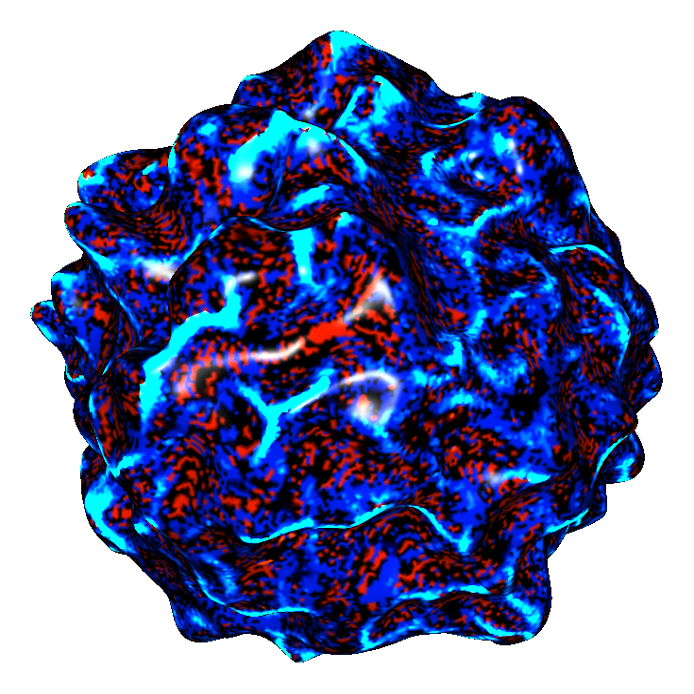
\includegraphics[width=0.22\figurewidth]{figures/sr_time_3_2.png} &
        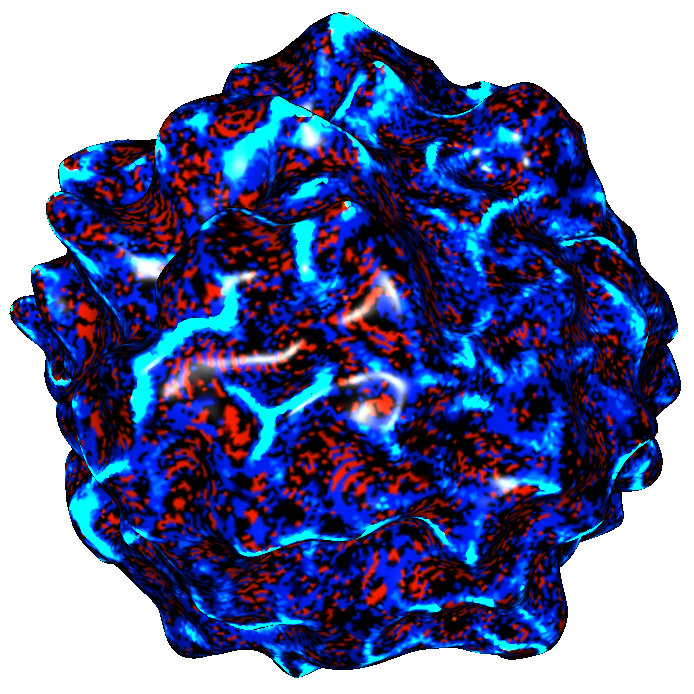
\includegraphics[width=0.22\figurewidth]{figures/sr_time_3_3.png} \\
    };
    \node[label, below=of time-3-1] {time step 1};
    \node[label, below=of time-3-2] {time step 4};
    \node[label, below=of time-3-3] {time step 8};

    \node[row label, at=(time.north west)] {time steps};

    \node[left=of time-1-1] {
        \rotatebox{90}{$t^\textnormal{HEATR}_\textnormal{max}$
                       vs. $t^{\ce{H2O2}}_\textnormal{max}$}
    };
    \node[left=of time-2-1] {
        \rotatebox{90}{$t^\textnormal{TEMP}_\textnormal{infl}$
                       vs. $t^\textnormal{HEATR}_\textnormal{max}$}
    };
    \node[left=of time-3-1] {
        \rotatebox{90}{$t^\textnormal{TEMP}_\textnormal{infl}$
                       vs. $t^{\ce{O}}_\textnormal{max}$}
    };
\end{tikzpicture}